\chapter{Phương pháp}
\label{chap:method}

Chương này mô tả chi tiết toàn bộ phương pháp luận và quy trình kỹ thuật của khóa luận theo đúng hành trình xử lý dữ liệu: mở đầu bằng bức tranh tổng thể của kiến trúc RC-Free đề xuất (Mục~\ref{sec:final-pipeline}); tiếp đến là quy trình xây dựng, làm sạch và phân chia tập dữ liệu nghiên cứu (Mục~\ref{sec:study-design}); các bước tiền xử lý chuyên sâu và cơ chế mã hóa ba nguồn thông tin đầu vào (Mục~\ref{sec:preprocessing}); tiến trình tiến hóa của khối hợp nhất đa phương thức từ ghép nối cơ bản đến kiến trúc RC-Free tinh gọn (Mục~\ref{sec:architecture-evolution}); phương pháp mô hình hóa chuỗi thời gian không đều tích hợp hàm mục tiêu sống còn Cox (Mục~\ref{sec:temporal-method}); và cuối cùng là khung đánh giá sống còn đa chiều (Mục~\ref{sec:survival-evaluation}).

\section{Tổng quan mô hình RC-Free}
\label{sec:final-pipeline}
Kiến trúc \textbf{RC-Free Pairwise Fusion (RC-Free)} được thiết kế để huấn luyện theo cơ chế đầu-cuối (end-to-end), nhằm ánh xạ chuỗi dữ liệu đa phương thức qua ba lần khám của mỗi cá thể thành một chỉ số log-nguy cơ $\eta_i \in \mathbb R$ duy nhất. Hình~\ref{fig:overall} phác họa bốn giai đoạn xử lý cốt lõi của mô hình:
\begin{enumerate}
\item \emph{Mã hóa từng nguồn dữ liệu}: Tại mỗi lần khám $t\in\{1,2,3\}$, thể tích MRI 3D được đưa qua mạng ResNet-18 3D để tạo vectơ đặc trưng $M_t\in\mathbb R^{128}$; các đặc trưng radiomics sau bước nén PCA đi qua khối MLP để tạo $R_t\in\mathbb R^{64}$; đồng thời các điểm lâm sàng kèm mặt nạ chỉ báo dữ liệu thiếu đi qua MLP để tạo $C_t\in\mathbb R^{64}$.
\item \emph{Hợp nhất theo cặp bằng CP và phần dư có cổng (RC-Free)}: Khối hợp nhất đặt MRI làm nút trung tâm kết nối để tính toán hai tương tác song tuyến MRI--Radiomics (MR) và MRI--Lâm sàng (MC) thông qua phân rã tensor CP hạng $Q=8$. Bốn nhánh phần dư có cổng điều tiết động truyền dẫn thông tin tương tác trở lại bồi đắp cho biểu diễn gốc để tạo thành bộ ba $(M_{\rm out}, R_{\rm out}, C_{\rm out})$; các vectơ này sau đó được ghép nối (256 chiều) và chiếu qua $\operatorname{MLP}_{\rm out}$ thành biểu diễn hợp nhất $F_t\in\mathbb R^{128}$ cho lần khám thứ $t$.
\item \emph{Tổng hợp biểu diễn theo trục thời gian}: Chuỗi đặc trưng $(F_1, F_2, F_3)$ cùng khoảng thời gian thực tế biến thiên giữa các lần chụp $(\Delta t_2, \Delta t_3)$ được đưa qua mạng T-LSTM kết hợp cơ chế chú ý (attention) cộng để tổng hợp thành một vectơ biểu diễn dọc duy nhất $z\in\mathbb R^{128}$.
\item \emph{Ước lượng nguy cơ sống còn}: Khối MLP đầu ra ánh xạ vectơ biểu diễn dọc $z$ thành điểm log-nguy cơ $\eta_i$, được tối ưu hóa trực tiếp bằng hàm mất mát đối log-hợp lý riêng phần Cox và đánh giá khách quan qua các thước đo C-index, Kaplan--Meier và IPCW-AUC.
\end{enumerate}

\begin{figure}[H]
\centering
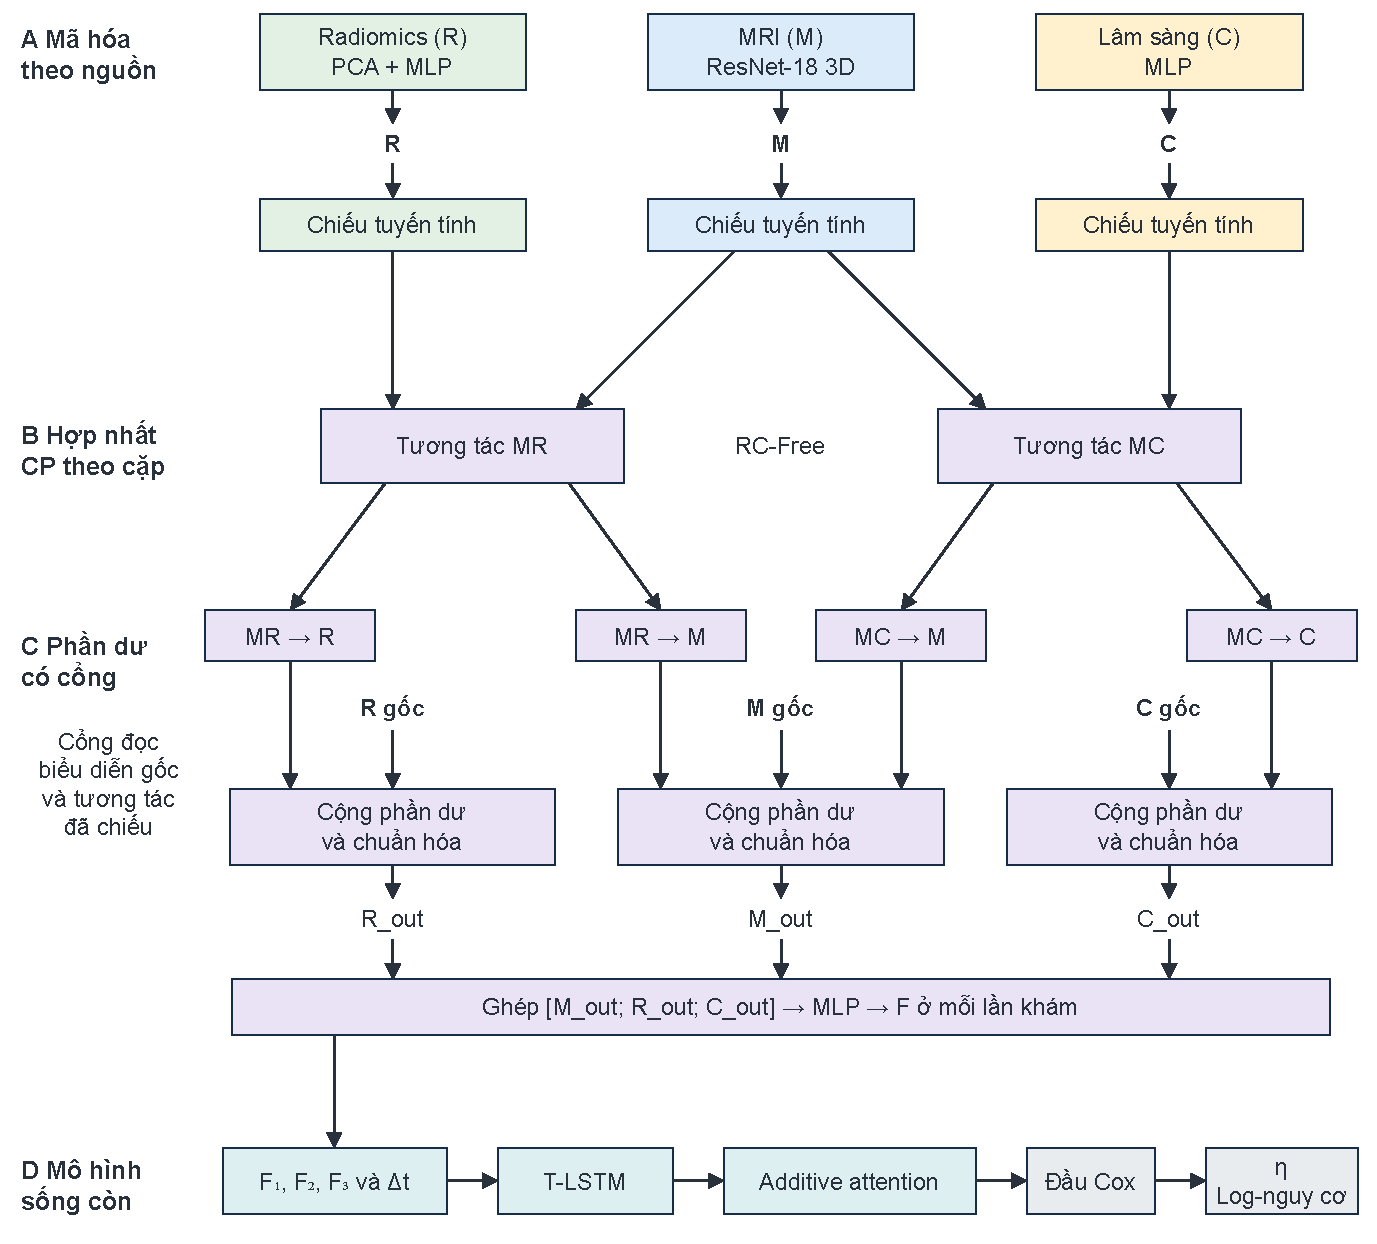
\includegraphics[width=\textwidth]{image/final-pipeline.pdf}
\caption{Sơ đồ quy trình xử lý tổng thể của mô hình RC-Free}
\label{fig:overall}
\end{figure}
\FloatBarrier

Sơ đồ tổng hợp đầy đủ từ dữ liệu thô đến đánh giá sống còn được đặt tại Hình~\ref{fig:master-pipeline}, Phụ lục~\ref{app:master-pipeline}.

\section{Thiết kế nghiên cứu và xây dựng dữ liệu}
\label{sec:study-design}

\subsection{Chọn mẫu và chuỗi ba lần chụp MRI}
Toàn bộ dữ liệu trong nghiên cứu này được trích xuất từ cơ sở dữ liệu của sáng kiến ADNI \cite{weiner2015impact,jack2008adnimri} trải dài qua ba giai đoạn gồm ADNI1, ADNIGO và ADNI2. Đối với mỗi người tham gia (được định danh duy nhất thông qua mã \texttt{RID}), tôi xác định lần khám ban đầu sớm nhất mang mã \texttt{bl} và có chẩn đoán xác nhận MCI (mã 2 trong trường \texttt{DXSUM.DIAGNOSIS}) \cite{adnidxsum}. Gọi $b_i$ là mốc thời gian khám ban đầu, tôi thiết lập \emph{mốc xét điều kiện chọn mẫu} là $L_i = b_i + 18$ tháng lịch.

Để bảo đảm mọi cá thể bước vào giai đoạn theo dõi sau mốc $L_i$ đều đang trong trạng thái chưa tiến triển bệnh, người tham gia sẽ bị loại trừ nếu đã có chẩn đoán sa sút trí tuệ (mã 3 trong \texttt{DXSUM.DIAGNOSIS}) \cite{adnidxsum}, hoặc có điểm MMSE $<24$, hoặc CDR-global $\geq 1$ tại bất kỳ thời điểm nào trước hoặc đúng mốc $L_i$. Thêm vào đó, mỗi người bệnh bắt buộc phải có ít nhất một lần đánh giá nhận thức lâm sàng hợp lệ sau mốc $L_i$ để làm căn cứ xác định kết cục theo dõi.

Kế thừa thiết kế ba lần chụp trong 18 tháng của Aghajanian và cộng sự \cite{aghajanian2025longitudinal}, tôi tiến hành chọn lọc ba ảnh MRI nằm trong cửa sổ $[b_i, L_i]$ sau khi đã gom cụm các lần chụp cách nhau tối thiểu hai tháng. Trong trường hợp một đợt khám có nhiều lần chụp lặp lại, quy trình ưu tiên lựa chọn ảnh chụp chính (primary scan) hơn ảnh chụp phụ, sau đó xếp hạng dựa trên tổ hợp nhãn tiền xử lý chuẩn của ADNI (giai đoạn ADNI1 ưu tiên nhãn \texttt{GradWarp + B1 + N3 + Scaled}; giai đoạn ADNIGO/ADNI2 ưu tiên nhãn \texttt{GradWarp + N3m}\footnote{Chi tiết các mức hiệu chỉnh ảnh MRI của ADNI: \url{https://adni.loni.usc.edu/data-samples/adni-data/neuroimaging/mri/mri-pre-processing/}.}). Nếu một cá thể có nhiều hơn ba đợt chụp hợp lệ, thuật toán sẽ tự động chọn lần đầu tiên, lần cuối cùng và lần trung gian có thời điểm gần trung điểm thời gian nhất, qua đó bảo đảm trật tự thời gian $s_{i1} < s_{i2} < s_{i3} \leq L_i$.

Như được minh họa ở Hình~\ref{fig:cohort}, từ 899 cá thể ban đầu có dữ liệu MRI liên kết định danh thành công, quy trình sàng lọc đã thu được chính xác \textbf{359 người tham gia} với 1077 thể tích ảnh MRI 3D (bao gồm 78 người từ ADNI1, 80 người từ ADNIGO và 201 người từ ADNI2), ghi nhận 106 ca xảy ra biến cố tiến triển và 253 ca kiểm duyệt phải.

\begin{figure}[H]
\centering
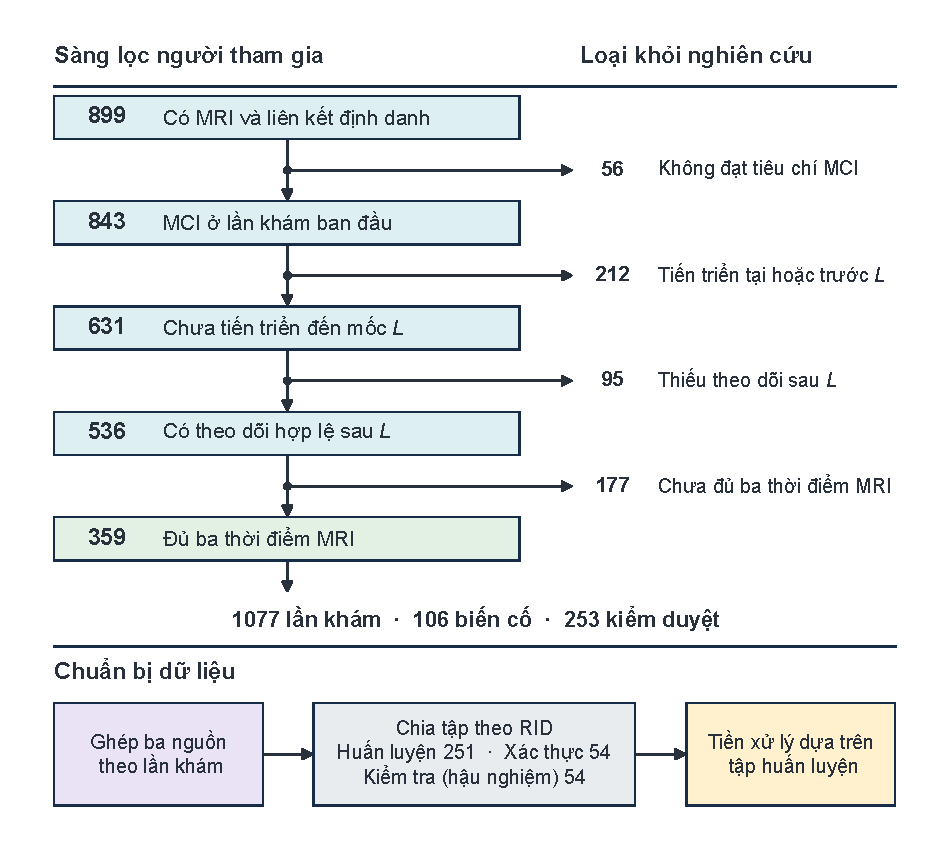
\includegraphics[width=\textwidth]{image/cohort-construction.pdf}
\caption{Quy trình xây dựng và chọn lọc nhóm nghiên cứu dọc}
\label{fig:cohort}
\end{figure}

\subsection{Biến cố, mốc thời gian và lưu ý về sai lệch thời gian bất tử}
\label{sec:evaluation-scope}
Theo tiêu chí lâm sàng của Aghajanian và cộng sự \cite{aghajanian2025longitudinal}, biến cố tiến triển được ghi nhận tại lần thăm khám hợp lệ đầu tiên sau mốc $L_i$ thỏa mãn điều kiện có điểm MMSE $<24$ hoặc CDR-global $\geq 1$. Nếu đến hết thời gian theo dõi mà người tham gia vẫn chưa từng vượt qua ngưỡng này, họ được ghi nhận là kiểm duyệt phải tại lần khám hợp lệ cuối cùng. Thời gian sống còn $t_i$ (đơn vị tính theo năm) được đo lường từ ngày chụp MRI lần thứ ba ($p_i = s_{i3}$) đến ngày ghi nhận biến cố hoặc ngày kiểm duyệt ($o_i$):
\begin{equation}
 t_i=\frac{o_i-p_i}{365.25},\qquad
 \delta_i=\begin{cases}1,&\text{nếu ghi nhận biến cố},\\0,&\text{nếu bị kiểm duyệt phải}.\end{cases}
 \label{eq:survival-target}
\end{equation}

Khi phân tích và diễn giải phương trình~(\ref{eq:survival-target}), một khía cạnh phương pháp luận hết sức quan trọng cần được lưu ý là khoảng chênh lệch thời gian giữa ngày chụp MRI lần ba $p_i$ và mốc xét điều kiện chọn mẫu $L_i$ (tháng thứ 18). Cụ thể, trong 359 người của bộ dữ liệu, có tới 356 người đã hoàn thành lần chụp MRI thứ ba trước mốc $L_i$, với khoảng cách thời gian $L_i - p_i$ có trung vị là 186 ngày (khoảng tứ phân vị từ 169 đến 197 ngày). Giả sử một người bệnh chụp MRI lần ba ở tháng thứ 12 ($p_i$) nhưng đến tháng thứ 18 ($L_i$) mới xét điều kiện đưa vào nghiên cứu: do quy trình chọn mẫu đã chủ động loại trừ toàn bộ những ai bị suy giảm nhận thức trước hoặc tại tháng thứ 18, nên bất kỳ cá thể nào còn hiện diện trong tập dữ liệu đều chắc chắn không thể xảy ra biến cố trong khoảng thời gian từ tháng 12 đến tháng 18. Trong dịch tễ học và thống kê y sinh, khoảng thời gian bảo đảm an toàn nhân tạo từ $p_i$ đến $L_i$ này được định nghĩa là ``thời gian bất tử'' — tức khoảng thời gian mà đối tượng nghiên cứu không thể gặp biến cố do chính quy tắc sàng lọc mẫu tạo ra. Do đó, việc cộng dồn khoảng thời gian này vào $t_i$ sẽ gây ra hiện tượng \emph{sai lệch thời gian bất tử} (immortal time bias) \cite{suissa2008immortal} nếu chúng ta xem mô hình như một công cụ dự báo tiến cứu tức thời ngay tại thời điểm chụp $p_i$. Vì lý do đó, các kết quả thực nghiệm trong khóa luận được diễn giải một cách chặt chẽ cho bài toán xếp hạng nguy cơ hồi cứu trên nhóm người bệnh đã được xác định là duy trì ổn định đến hết mốc $L_i$.

Ngoài ra, đầu ra $\eta_i$ từ mô hình rủi ro tỷ lệ Cox là điểm xếp hạng tương đối nhằm xác định thứ tự rủi ro tiến triển giữa các người bệnh với nhau. Nếu muốn chuyển đổi điểm số này thành xác suất tiến triển cụ thể theo thời gian (dưới dạng tỷ lệ phần trăm tại các thời hạn nhất định) cho từng cá thể, mô hình cần ước lượng bổ sung hàm nguy cơ tích lũy nền $H_0(t)$ \cite{cox1972regression}, nội dung này sẽ được tôi thảo luận chi tiết ở Chương~\ref{chap:discussion}.

\subsection{Phân chia dữ liệu và kiểm soát rò rỉ thông tin}
\label{sec:data-split}
Nhằm ngăn chặn triệt để nguy cơ rò rỉ dữ liệu giữa các tập, việc phân chia dữ liệu được thực hiện cố định theo mã định danh người bệnh (\texttt{RID}): tập huấn luyện gồm 251 người (74 ca biến cố), tập xác thực gồm 54 người (16 ca biến cố) và tập kiểm tra hậu nghiệm gồm 54 người (16 ca biến cố), bảo đảm tỷ lệ biến cố duy trì ổn định trong khoảng 29.5--29.6\% trên cả ba phân tập. Tập xác thực được sử dụng độc quyền cho việc tìm kiếm siêu tham số và lựa chọn kiến trúc tối ưu; trong khi đó, tập kiểm tra chỉ được đưa vào đánh giá hậu nghiệm độc lập sau khi mô hình đã được cố định hoàn toàn.

Đặc biệt, toàn bộ các tham số tiền xử lý dữ liệu dạng bảng (bao gồm giá trị trung vị dùng để điền khuyết, giá trị trung bình cùng độ lệch chuẩn chuẩn hóa, và ma trận chiếu PCA) đều chỉ được tính toán và khớp trên tập huấn luyện, sau đó áp dụng một chiều sang hai tập còn lại. Các biến đặc trưng đầu vào tuyệt đối không chứa nhãn chẩn đoán bệnh, trạng thái biến cố hay thời gian sống còn.

Mỗi lần chụp MRI được liên kết đồng bộ với lần đánh giá lâm sàng hợp lệ gần nhất nằm trong cửa sổ thời gian $\pm 90$ ngày. Về mặt thực tế, trong số 359 người bệnh có 57 trường hợp có điểm MMSE hoặc CDR lấy từ lần đo diễn ra sau ngày chụp MRI cuối $p_i$ (song vẫn bảo đảm diễn ra trước thời điểm kết cục $o_i$); giới hạn này được tôi ghi nhận và phân tích cụ thể ở Mục~\ref{sec:study-limitations}. Bảng~\ref{tab:baseline-characteristics} tổng hợp chi tiết đặc điểm nhân khẩu học, điểm nhận thức ban đầu và khoảng cách giữa các lần khám của ba tập dữ liệu; các kiểm định thống kê so sánh giữa ba tập đều ghi nhận $p > 0.05$, khẳng định tính cân đồng nhất của các phân tập.

\begin{landscape}
\begin{table}[p]
\centering\small
\caption[Đặc điểm người tham gia tại MRI đầu]{Đặc điểm người tham gia tại MRI đầu, chia theo tập và trạng thái kết cục.}
\label{tab:baseline-characteristics}
\setlength{\tabcolsep}{2pt}
\begin{tabular}{@{}lrrrrrrr@{}}
\toprule
& \multicolumn{2}{c}{Huấn luyện ($N=251$)} & \multicolumn{2}{c}{Xác thực ($N=54$)} & \multicolumn{2}{c}{Kiểm tra ($N=54$)} & $p$ \\
\cmidrule(lr){2-3}\cmidrule(lr){4-5}\cmidrule(lr){6-7}
Đặc điểm & $\delta=0$ & $\delta=1$ & $\delta=0$ & $\delta=1$ & $\delta=0$ & $\delta=1$ & \\
\midrule
Số người & 177 & 74 & 38 & 16 & 38 & 16 & -- \\
Tuổi tại MRI đầu (năm) & $71.64 \pm 7.5390$ & $73.41 \pm 7.1692$ & $71.29 \pm 8.6426$ & $74.86 \pm 5.6415$ & $70.03 \pm 7.5755$ & $72.74 \pm 6.7222$ & 0.4895 \\
Nam, n (\%) & 96 (54.24) & 49 (66.22) & 23 (60.53) & 10 (62.50) & 28 (73.68) & 9 (56.25) & 0.3367 \\
Học vấn (năm) & $16.37 \pm 2.7171$ & $16.61 \pm 2.5846$ & $15.32 \pm 2.5691$ & $17.00 \pm 2.5298$ & $17.00 \pm 2.6304$ & $16.19 \pm 2.9489$ & 0.1465 \\
MMSE ban đầu & $28.57 \pm 1.3799$ (53) & $27.22 \pm 1.7746$ (36) & $28.54 \pm 1.1266$ (13) & $27.75 \pm 1.4880$ (8) & $28.25 \pm 1.5275$ (16) & $26.83 \pm 2.0412$ (6) & 0.8688 \\
CDR-global ban đầu & $0.44 \pm 0.1613$ (52) & $0.49 \pm 0.0833$ (36) & $0.38 \pm 0.2193$ (13) & $0.44 \pm 0.1768$ (8) & $0.47 \pm 0.1250$ (16) & $0.50 \pm 0.0000$ (6) & 0.2060 \\
CDR-SB ban đầu & $0.92 \pm 0.5721$ (52) & $1.68 \pm 0.9573$ (36) & $1.04 \pm 0.8026$ (13) & $1.56 \pm 1.1476$ (8) & $1.28 \pm 0.9123$ (16) & $1.67 \pm 0.9309$ (6) & 0.7260 \\
$s_2-s_1$ (ngày) & $120.47 \pm 40.5683$ & $134.04 \pm 45.0152$ & $131.76 \pm 41.8372$ & $129.50 \pm 46.4672$ & $124.34 \pm 42.4470$ & $137.50 \pm 44.4627$ & 0.4313 \\
$s_3-s_1$ (ngày) & $305.12 \pm 44.1559$ & $313.04 \pm 42.8334$ & $307.32 \pm 34.0271$ & $312.19 \pm 75.3819$ & $312.08 \pm 55.0550$ & $315.50 \pm 38.4430$ & 0.8898 \\
$t_i$ (năm), TB $\pm$ SD & $5.11 \pm 3.9055$ & $3.41 \pm 2.7858$ & $5.59 \pm 4.7319$ & $3.85 \pm 3.2066$ & $5.51 \pm 4.3420$ & $3.11 \pm 2.5391$ & 0.8713 \\
$t_i$ (năm), trung vị [Q1; Q3] & 3.64 [2.02; 7.54] & 2.09 [1.66; 4.42] & 3.92 [2.05; 6.73] & 3.69 [1.44; 4.88] & 4.06 [2.02; 8.20] & 2.42 [1.54; 3.64] & -- \\
\bottomrule
\end{tabular}
\par\vspace{6pt}
\begin{minipage}{0.96\linewidth}\small
$\delta=0$ biểu thị kiểm duyệt và $\delta=1$ biểu thị biến cố. Trừ các dòng có ghi riêng, bảng trình bày trung bình $\pm$ SD mẫu. Với MMSE và CDR, số trong ngoặc là số quan sát hợp lệ trước khi điền thiếu. Tỷ lệ nam tính trên số người có thông tin giới tính. Tuổi được ước tính từ tháng và năm sinh, quy ước ngày sinh là ngày 15. Các biến nhân khẩu học lấy từ bản ghi hợp lệ gần MRI đầu nhất, tính đến ngày chụp. Các điểm MMSE và CDR được ghép trong cửa sổ $\pm90$ ngày. Giá trị $p$ mô tả khác biệt giữa ba tập, gộp cả hai trạng thái kết cục, theo kiểm định Kruskal--Wallis cho biến định lượng và kiểm định $\chi^2$ cho giới tính. $s_3-s_1$ là khoảng thời gian từ MRI đầu đến MRI cuối. $t_i$ là thời gian từ MRI cuối đến biến cố hoặc kiểm duyệt.
\end{minipage}
\end{table}
\end{landscape}


\section{Tiền xử lý và mã hóa ba nguồn dữ liệu}
\label{sec:preprocessing}
Hình~\ref{fig:input-three-sources} minh họa trực quan ba nguồn thông tin được liên kết chặt chẽ tại mỗi lần thăm khám trước khi đưa vào ba bộ mã hóa độc lập.

\begin{figure}[H]
\centering
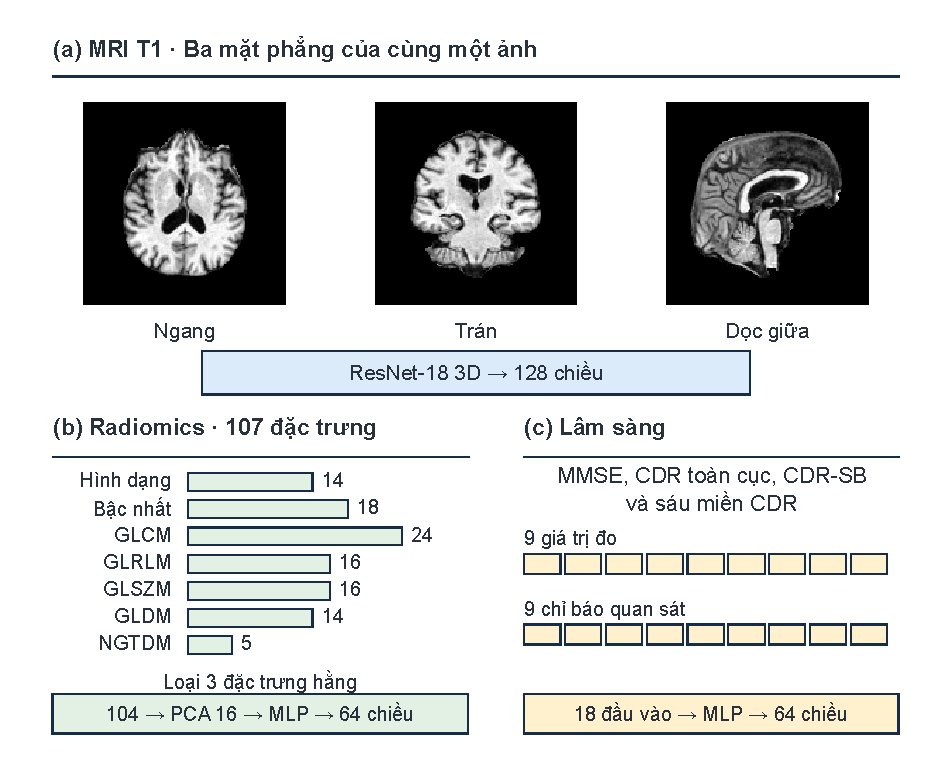
\includegraphics[width=\textwidth]{image/input-three-sources.pdf}
\caption[Minh họa ba nguồn dữ liệu đầu vào và các biểu diễn đặc trưng]{Ba nguồn dữ liệu đầu vào và biểu diễn tương ứng. Ba mặt phẳng MRI được tác giả trích từ cùng một ảnh T1 của ADNI sau tiền xử lý \cite{jack2008adnimri}.}
\label{fig:input-three-sources}
\end{figure}

\subsection{Nhánh MRI 3D và bộ mã hóa dùng chung}
Trong xử lý ảnh cộng hưởng từ não bộ 3D dọc, chỉ một chuyển động nghiêng đầu nhẹ của người bệnh giữa các lần chụp cũng khiến cùng một cấu trúc giải phẫu (như hồi hải mã) rơi vào các tọa độ không gian khác nhau, dễ dẫn đến việc mô hình nhầm lẫn giữa sai lệch tư thế và sự teo não bệnh lý thực sự. Mặt khác, thang cường độ sáng trên ảnh MRI mang tính quy ước tương đối và thường có độ lệch giữa các máy quét khác nhau \cite{nyul1999standardizing}. Vì vậy, chuỗi tiền xử lý (Hình~\ref{fig:mri-preprocessing}) được tôi thiết lập với năm bước tuần tự nhằm đồng nhất tư thế không gian, kích thước lưới voxel và chuẩn hóa thang cường độ mà không làm biến dạng hình học giải phẫu tự nhiên của não bộ:

\begin{figure}[H]
\centering
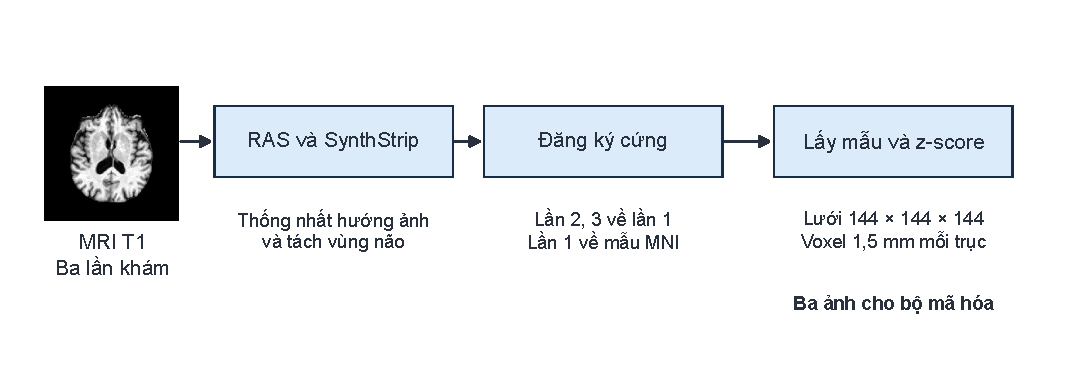
\includegraphics[width=\textwidth]{image/mri-preprocessing.pdf}
\caption[Quy trình tiền xử lý chuỗi ảnh MRI T1 dọc]{Quy trình tiền xử lý chuỗi ảnh MRI T1 dọc. Hình dùng lại một lát cắt ADNI ở Hình~\ref{fig:input-three-sources} để minh họa các bước.}
\label{fig:mri-preprocessing}
\end{figure}

\begin{enumerate}
\item \emph{Chuẩn hóa hướng trục và bóc tách hộp sọ}: Đưa toàn bộ thể tích MRI về chung quy ước không gian giải phẫu chuẩn RAS (\emph{Right--Anterior--Superior}), sau đó áp dụng mô hình học sâu SynthStrip \cite{hoopes2022synthstrip} để loại bỏ triệt để phần hộp sọ, mô da đầu và sinh mặt nạ nhị phân toàn não (gán giá trị 1 cho vùng trong não, 0 cho vùng ngoài não; không phân tách riêng rẽ chất xám, chất trắng hay dịch não tủy).
\item \emph{Căn chỉnh cứng giữa các lần khám và quy chiếu về mẫu MNI}: Ảnh chụp ở lần khám thứ hai và thứ ba của mỗi người được đăng ký không gian về ảnh lần khám đầu tiên thông qua \emph{phép biến đổi cứng} (rigid registration) 6 bậc tự do (gồm 3 bậc tịnh tiến và 3 bậc quay, có dạng $\mathbf{x}'=\mathbf{R}\mathbf{x}+\mathbf{t}$). Tiếp theo đó, ảnh lần đầu của mỗi người được căn chỉnh cứng về mẫu chuẩn quốc tế MNI152NLin2009cAsym \cite{mcgill2009icbm,fonov2009templates,fonov2011atlases} nhằm thiết lập hệ tọa độ giải phẫu chung giữa mọi cá thể (Hình~\ref{fig:mri-registration}). Quy trình này chủ động không áp dụng phép biến đổi affine co giãn hay biến dạng phi tuyến đàn hồi nhằm bảo tồn nguyên vẹn kích thước thể tích và hình thái thực của não bộ qua thời gian.
\item \emph{Lấy mẫu lại trên lưới voxel chung}: Đưa cả thể tích ảnh và mặt nạ não về lưới chuẩn kích thước $144\times144\times144$ voxel với độ phân giải đẳng hướng $1.5\text{ mm}$, sử dụng phép nội suy tuyến tính cho ảnh cường độ và phép nội suy láng giềng gần nhất cho mặt nạ nhằm bảo toàn tuyệt đối giá trị nhị phân $0/1$.
\item \emph{Chuẩn hóa thang cường độ trong vùng não}: Đối với từng ảnh riêng lẻ, các voxel nằm bên trong mặt nạ não được chuẩn hóa z-score theo công thức $z(v)=(I(v)-\mu)/\sigma$ (trong đó $\mu,\sigma$ được tính riêng trên tập voxel thuộc mặt nạ của chính ảnh đó) nhằm đưa phân bố độ sáng về trung bình 0 và phương sai 1; các voxel bên ngoài mặt nạ được gán bằng 0. Quy trình không can thiệp thêm bước hiệu chỉnh trường không đồng nhất N4 nhằm giữ trọn đặc tính tín hiệu gốc.
\end{enumerate}

\begin{figure}[H]
\centering
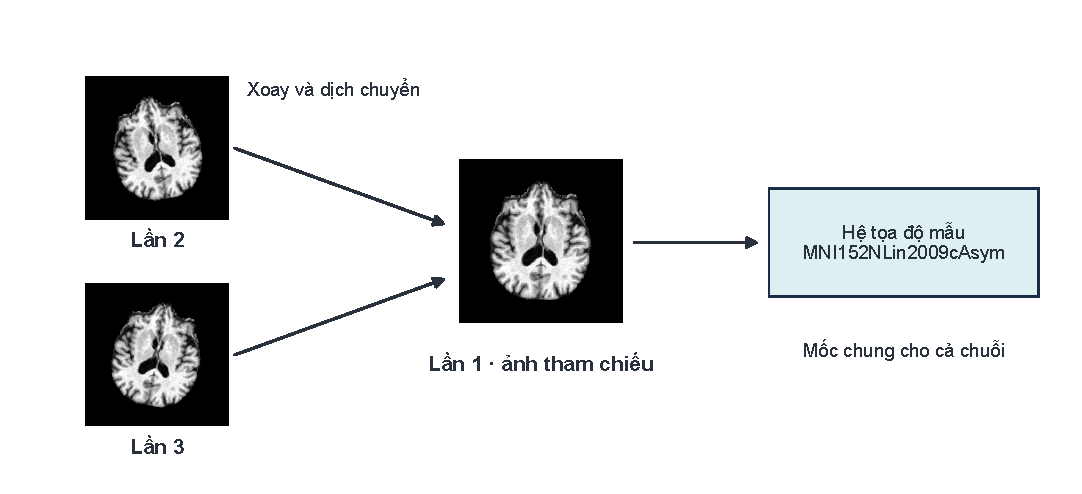
\includegraphics[width=\textwidth]{image/mri-registration.pdf}
\caption[Quy trình căn chỉnh không gian MRI giữa các lần khám và về mẫu MNI]{Căn chỉnh cứng giữa các lần khám và về mẫu MNI. Các tư thế được minh họa bằng cách xoay cùng một lát cắt ADNI ở Hình~\ref{fig:input-three-sources}.}
\label{fig:mri-registration}
\end{figure}

Sau khi hoàn tất tiền xử lý, toàn bộ ba ảnh MRI của mỗi người bệnh được đưa qua một bộ mã hóa dùng chung \textbf{ResNet-18 3D} được cài đặt dựa trên thư viện MONAI phiên bản 1.5.2\footnote{Mã nguồn MONAI: \url{https://github.com/Project-MONAI/MONAI/blob/1.5.2/monai/networks/nets/resnet.py}.} \cite{he2016deep,cardoso2022monai}, nạp trọn vẹn bộ trọng số và trạng thái BatchNorm tiền huấn luyện trên ảnh y khoa 3D từ MedicalNet \cite{chen2019med3d} (sau khi loại bỏ lớp phân loại đầu ra cũ) và tinh chỉnh toàn bộ mạng ngay từ vòng huấn luyện đầu tiên. Kiến trúc gồm bốn tầng tích chập 3D liên tiếp (với số kênh lần lượt là 64, 128, 256 và 512) kết hợp chuẩn hóa BatchNorm \cite{ioffe2015batchnorm} và hàm kích hoạt ReLU \cite{nair2010rectified}. Sau bước gộp trung bình toàn cục thành vectơ 512 chiều, một lớp chiếu tuyến tính $512\to128$ kết hợp hàm kích hoạt GELU \cite{hendrycks2016gelu}, kỹ thuật Dropout 0.20 \cite{srivastava2014dropout} và lớp chuẩn hóa LayerNorm \cite{ba2016layernorm} tạo ra vectơ biểu diễn giải phẫu $M_t\in\mathbb R^{128}$ cho từng thời điểm khám. Bảng~\ref{tab:mri-encoder-shapes} ở Phụ lục~\ref{app:mri-shapes} trình bày chi tiết kích thước bản đồ đặc trưng qua từng tầng.

\subsection{Nhánh đặc trưng Radiomics}
\label{sec:radiomics-pipeline}
Song hành cùng các đặc trưng học sâu trừu tượng từ CNN, nhánh radiomics tiến hành trích xuất hệ thống các chỉ số hình học và hoa văn kết cấu định lượng tường minh từ chính thể tích MRI và mặt nạ não bộ bằng thư viện PyRadiomics \cite{vangriethuysen2017computational}. Quy trình trích xuất gồm bốn bước chuẩn mực:
\begin{enumerate}
\item \emph{Trích xuất 107 đặc trưng trong thang $[0,1]$}: Khác với nhánh CNN tiếp nhận ảnh đã chuẩn hóa z-score, nhánh radiomics co giãn tuyến tính cường độ voxel trong mặt nạ của từng ảnh về đoạn $[0,1]$ và thực hiện rời rạc hóa với tùy chọn \texttt{binCount=64} \cite{pyradiomicsbins} trước khi trích xuất 107 đặc trưng thuộc 7 nhóm: hình dạng (14 biến), thống kê cường độ bậc nhất (18 biến) và 5 nhóm ma trận kết cấu không gian gồm GLCM, GLRLM, GLSZM, GLDM, NGTDM (75 biến), được tóm tắt ở Bảng~\ref{tab:radiomics-groups}.
\item \emph{Loại bỏ biến hằng}: Do toàn bộ cường độ ảnh đã được co giãn về đoạn chuẩn $[0,1]$, ba đặc trưng thống kê bậc nhất gồm \texttt{Minimum}=0, \texttt{Maximum}=1 và \texttt{Range}=1 trở thành các giá trị hằng số cố định ở mọi đối tượng và được loại bỏ, đưa số lượng đặc trưng về còn 104 biến.
\item \emph{Giảm chiều bằng PCA}: Để triệt tiêu hiện tượng đa cộng tuyến giữa 104 đặc trưng, tôi tiến hành chuẩn hóa z-score từng biến và khớp mô hình PCA \cite{jolliffe2016pca} duy nhất trên tập huấn luyện với ngưỡng giữ lại ít nhất 99\% tổng phương sai giải thích, qua đó thu được đúng 16 thành phần chính độc lập tại mỗi lần khám.
\item \emph{Mã hóa qua mạng MLP}: Vectơ 16 chiều sau đó được đưa qua khối MLP ($16\to128\to64$) tích hợp hàm kích hoạt GELU, Dropout 0.20 và LayerNorm để tạo thành vectơ biểu diễn $R_t\in\mathbb R^{64}$.
\end{enumerate}

\begin{table}[H]
\centering\small
\caption[Các nhóm đặc trưng radiomics]{Bảy nhóm đặc trưng radiomics trích từ ảnh và mặt nạ toàn não. Định nghĩa và ví dụ theo PyRadiomics \cite{pyradiomicsfeatures}. Số lượng lấy từ danh mục đặc trưng của khóa luận.}
\label{tab:radiomics-groups}
\begin{tabularx}{\linewidth}{@{}L{2.7cm}r Y Y@{}}
\toprule
Nhóm & Số lượng & Thông tin mô tả & Ví dụ \\
\midrule
Hình dạng & 14 & Hình học của mặt nạ não & Thể tích (MeshVolume), diện tích bề mặt (SurfaceArea) \\
Thống kê bậc nhất & 18 & Phân bố cường độ trong mặt nạ & Trung bình (Mean), phương sai (Variance), Entropy \\
GLCM & 24 & Quan hệ mức xám giữa các cặp voxel & Contrast, Correlation \\
GLRLM & 16 & Độ dài chuỗi voxel cùng mức xám theo hướng & ShortRunEmphasis, LongRunEmphasis \\
GLSZM & 16 & Kích thước vùng liên thông cùng mức xám & SmallAreaEmphasis, LargeAreaEmphasis \\
GLDM & 14 & Mức phụ thuộc cường độ giữa voxel và lân cận & DependenceEntropy, DependenceVariance \\
NGTDM & 5 & Chênh lệch cường độ với lân cận & Coarseness, Contrast, Busyness, Complexity, Strength \\
\midrule
Tổng & 107 & Còn 104 sau khi loại Maximum, Minimum và Range & PCA giữ 16 thành phần \\
\bottomrule
\end{tabularx}
\end{table}


\subsection{Nhánh dữ liệu lâm sàng và chỉ báo có dữ liệu}
Nhánh lâm sàng khai thác 9 biến số dự báo then chốt (Bảng~\ref{tab:clinical-inputs}), bao gồm ba điểm số tổng hợp (MMSE-total \cite{folstein1975mmse}, CDR-global, CDR-SB) và sáu điểm thành phần theo từng miền chức năng của thang CDR \cite{morris1993cdr}. Mọi giá trị bị khuyết thiếu đều được điền bằng giá trị trung vị của biến đó tại cùng lần khám trên tập huấn luyện (nếu toàn bộ lần khám đó bị thiếu thì sử dụng trung vị tính trên toàn tập huấn luyện), tiếp theo đó được chuẩn hóa theo kỳ vọng và độ lệch chuẩn của tập huấn luyện.

Do giá trị sau khi điền khuyết có thể trùng ngẫu nhiên với một số đo thực tế, mỗi biến lâm sàng được bổ sung thêm một \emph{chỉ báo nhị phân} (nhận giá trị 1 nếu có số đo thực tế, và 0 nếu bị khuyết trước khi điền), qua đó mở rộng không gian đầu vào từ 9 lên 18 chiều (Hình~\ref{fig:clinical-18}). Vectơ 18 chiều này được đưa qua khối MLP ($18\to64\to64$) kết hợp hàm kích hoạt GELU, Dropout 0.10 và LayerNorm để sinh ra biểu diễn lâm sàng $C_t\in\mathbb R^{64}$.

\begin{table}[H]
\centering\small
\caption[Chín biến lâm sàng đầu vào]{Chín giá trị trước khi chuẩn hóa, theo đúng thứ tự đầu vào của mô hình. MMSE theo Folstein và cộng sự \cite{folstein1975mmse}, CDR theo Morris \cite{morris1993cdr}. Mỗi giá trị có thêm một chỉ báo quan sát tương ứng.}
\label{tab:clinical-inputs}
\begin{tabularx}{\linewidth}{@{}r L{3.6cm}Y@{}}
\toprule
Vị trí & Biến lâm sàng & Ý nghĩa \\
\midrule
1 & MMSE-total & Tổng điểm đánh giá nhận thức, thang 0--30 \\
2 & CDR-global & Mức độ suy giảm nhận thức và chức năng tổng thể \\
3 & CDR-SB & Tổng điểm của sáu miền CDR, thang 0--18 \\
4 & CDR: trí nhớ & Khả năng ghi nhớ và nhớ lại thông tin \\
5 & CDR: định hướng & Nhận biết thời gian, địa điểm và hoàn cảnh \\
6 & CDR: phán đoán & Khả năng phán đoán và giải quyết vấn đề \\
7 & CDR: cộng đồng & Khả năng tham gia hoạt động ngoài gia đình \\
8 & CDR: gia đình và sở thích & Khả năng thực hiện công việc tại nhà và duy trì sở thích \\
9 & CDR: tự chăm sóc & Mức độc lập trong chăm sóc bản thân \\
\bottomrule
\end{tabularx}
\end{table}


\begin{figure}[H]
\centering
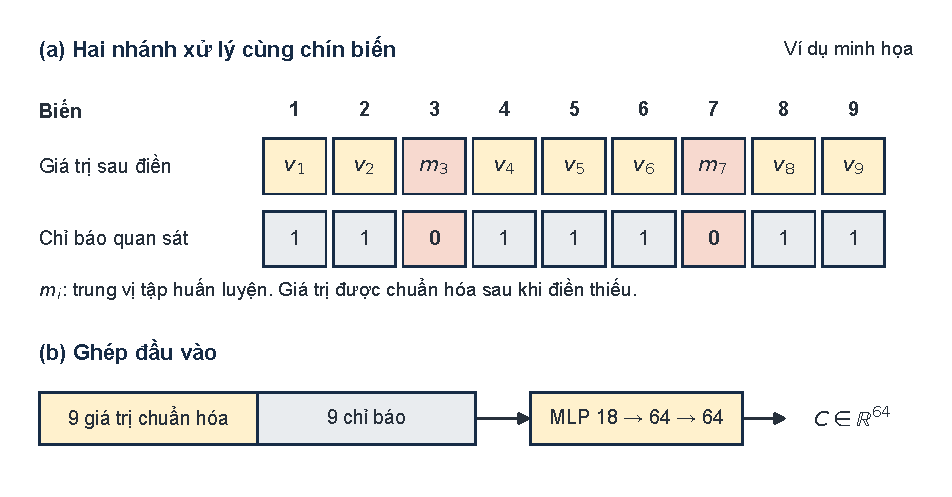
\includegraphics[width=\textwidth]{image/clinical-18-inputs.pdf}
\caption{Quy trình mở rộng chín biến lâm sàng thành 18 chiều đầu vào}
\label{fig:clinical-18}
\end{figure}

\section{Hợp nhất đa phương thức: từ ghép nối đến RC-Free}
\label{sec:architecture-evolution}
Mục này trình bày quá trình phát triển có hệ thống của khối hợp nhất ba nguồn biểu diễn $(M_t, R_t, C_t)$ theo đúng trình tự kiểm chứng thực nghiệm của khóa luận: từ việc xây dựng các mô hình tham chiếu chỉ dùng ảnh MRI (Mục~\ref{sec:ref-models}), đối chứng phương thức ghép nối trực tiếp với tương tác tích ngoài song tuyến (Mục~\ref{sec:pair-fusion}), nén lớp tương tác bằng kỹ thuật phân rã CP (Mục~\ref{sec:cp-method}), cho đến việc hoàn thiện cơ chế truyền phần dư có cổng điều tiết và cấu trúc tinh gọn RC-Free (Mục~\ref{sec:gated-routing}).

\subsection{Các mô hình tham chiếu trên dữ liệu MRI}
\label{sec:ref-models}
Nhằm đánh giá chính xác giá trị gia tăng của thông tin dọc và tạo cơ sở đối chiếu vững chắc với các nghiên cứu tiền nhiệm, khóa luận xây dựng một chuỗi các mô hình tham chiếu chỉ sử dụng dữ liệu MRI (bao gồm mô hình chỉ dùng ảnh MRI cuối cùng, mô hình chuỗi 3 ảnh MRI với T-LSTM, và mô hình kết hợp T-LSTM với attention) song hành cùng một bản tái lập có điều chỉnh quy trình CNN--PCA--T-LSTM của Aghajanian và cộng sự \cite{aghajanian2025longitudinal}. Trong bản tái lập này, mạng CNN trên nền tảng TensorFlow tiếp nhận ảnh MRI kích thước $128^3$ và xuất ra vectơ 512 chiều; phép biến đổi PCA được khớp trên tập huấn luyện với ngưỡng giữ lại 99\% phương sai (không chuẩn hóa thang đo hay làm trắng) trước khi đưa vào mạng T-LSTM có trạng thái ẩn 64 chiều. Bảng~\ref{tab:reference-methods} phân định rõ các điểm tương đồng và khác biệt giữa công trình gốc, bản tái lập và mô hình chính của khóa luận. Toàn bộ nhóm mô hình chính được triển khai đồng bộ trên PyTorch, MONAI và scikit-learn \cite{paszke2019pytorch,cardoso2022monai,pedregosa2011sklearn}; sự khác biệt về thuật toán tối ưu và cỡ lô của bản tái lập CNN--PCA--T-LSTM được chuẩn hóa để đối chiếu công bằng thông qua chỉ số C-index.

\begin{table}[H]
\centering\small
\caption[Phân biệt công trình gốc, bản tái lập có điều chỉnh và phương pháp chính]{So sánh dữ liệu, cấu hình và vai trò của ba phương pháp.}
\label{tab:reference-methods}
\begin{tabularx}{\textwidth}{@{}L{3.2cm}Y Y@{}}
\toprule
\textbf{Phương pháp} & \textbf{Dữ liệu và tiền xử lý} & \textbf{Mô hình và vai trò} \\
\midrule
Aghajanian gốc \cite{aghajanian2025longitudinal} & 228 người có MCI; SPM12, mô não và radiomics chất xám & CNN--PCA--T-LSTM; huấn luyện hai bước; công trình tham chiếu \\
Bản tái lập có điều chỉnh & 359 người; ảnh MRI cố định đổi kích thước về $128^3$ & CNN/PCA theo lần khởi tạo; T-LSTM 64; đối chứng triển khai \\
RC-Free Pairwise & 359 người; MRI $144^3$, radiomics toàn não, lâm sàng 18 chiều & MedicalNet; CP MR/MC; phần dư có cổng; T-LSTM 128; mô hình chính \\
\bottomrule
\end{tabularx}
\end{table}

\subsection{Đối chứng ghép nối và hợp nhất tương tác tích ngoài}
\label{sec:pair-fusion}
Khi kết hợp đồng thời cả ba luồng biểu diễn đặc trưng $(M_t\in\mathbb R^{128}, R_t\in\mathbb R^{64}, C_t\in\mathbb R^{64})$, mô hình cơ sở trực quan nhất là \textbf{đối chứng ghép nối (Concatenation)}: giữ nguyên ba bộ mã hóa, nối trực tiếp ba vectơ thành một vectơ 256 chiều rồi đưa qua lớp $\operatorname{MLP}_{\rm out}$ (gồm tầng tuyến tính $256\to128$, GELU, Dropout 0.20 và LayerNorm) để tạo biểu diễn $F_t\in\mathbb R^{128}$ cho khối thời gian (Hình~\ref{fig:concat-baseline}):
\begin{equation}
 F_t=\operatorname{MLP}_{\rm out}(M_t\concat R_t\concat C_t),\qquad
 M_t\concat R_t\concat C_t\in\mathbb R^{256},\quad F_t\in\mathbb R^{128}.
 \label{eq:concat}
\end{equation}

\begin{figure}[H]
\centering
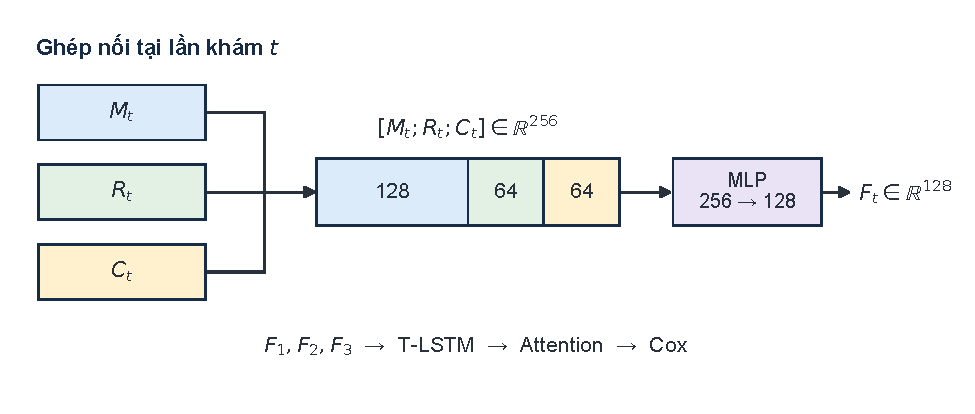
\includegraphics[width=\textwidth]{image/concat-baseline.pdf}
\caption[Mô hình đối chứng ghép nối]{Luồng tính toán của mô hình đối chứng ghép nối ba nguồn.}
\label{fig:concat-baseline}
\end{figure}

Ở phương thức ghép nối đơn thuần, mô hình hoàn toàn phó mặc việc khám phá mối quan hệ chéo giữa các phương thức cho các lớp biểu diễn phía sau. Để khắc phục hạn chế này và mô hình hóa tường minh tương tác song tuyến giữa từng cặp nguồn ngay trước bước ghép nối~(\ref{eq:concat}), tôi xây dựng biến thể \textbf{tích ngoài đầy đủ (Full Outer-Product)} nhằm bổ sung ba cặp tương tác song tuyến MR, MC và RC. Trước hết, ba phép chiếu tuyến tính không dùng hệ số chệch được áp dụng để giảm số chiều của từng biểu diễn gốc, qua đó khống chế kích thước không gian tích ngoài:
\begin{equation}
 \widetilde M\in\mathbb R^{32},\qquad
 \widetilde R\in\mathbb R^{32},\qquad
 \widetilde C\in\mathbb R^{16}.
 \label{eq:input-projection}
\end{equation}

Với mỗi cặp $k\in\{\mathrm{MR},\mathrm{MC},\mathrm{RC}\}$, ký hiệu hai vectơ đã giảm chiều là $x\in\mathbb R^{d_x}$ và $y\in\mathbb R^{d_y}$. Mô hình tính ma trận tích ngoài $xy^\top \in \mathbb R^{d_x\times d_y}$, trải phẳng thành vectơ (1024 chiều cho cặp MR; 512 chiều cho hai cặp MC và RC) rồi đưa qua khối MLP hai lớp kết hợp GELU, Dropout 0.10 và LayerNorm (với quy mô mạng tương ứng là MR: $1024\to128\to64$; MC: $512\to128\to64$; RC: $512\to64\to32$), như minh họa ở Hình~\ref{fig:mr-outer-product}. Khi áp dụng đầy đủ cả ba cặp, sáu nhánh truyền dẫn sẽ chiếu ngược các đặc trưng tương tác về kích thước của từng phương thức đích để cộng dồn vào biểu diễn gốc trước khi đưa qua cùng lớp $\operatorname{MLP}_{\rm out}$ (Hình~\ref{fig:pair-update-routes}).

\begin{figure}[H]
\centering
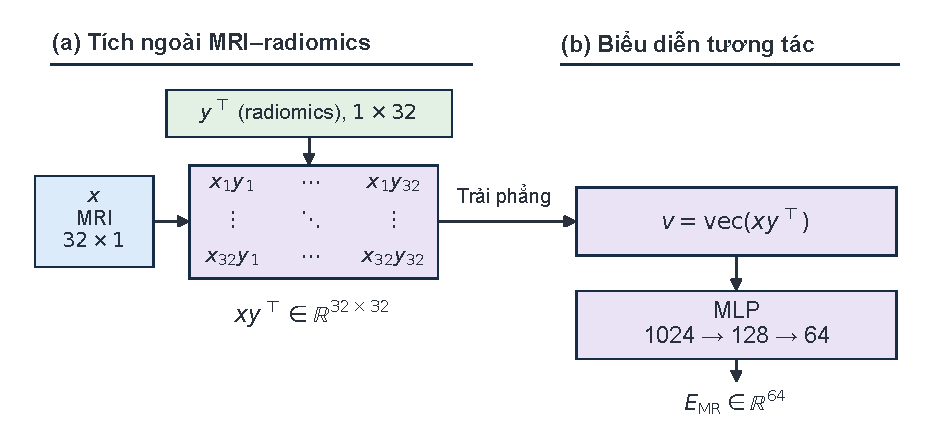
\includegraphics[width=\textwidth]{image/mr-outer-product.pdf}
\caption[Phép tích ngoài đầy đủ và khối MLP tương tác]{Phép tích ngoài đầy đủ và khối MLP tương tác (minh họa cho cặp MR)}
\label{fig:mr-outer-product}
\end{figure}

\begin{figure}[H]
\centering
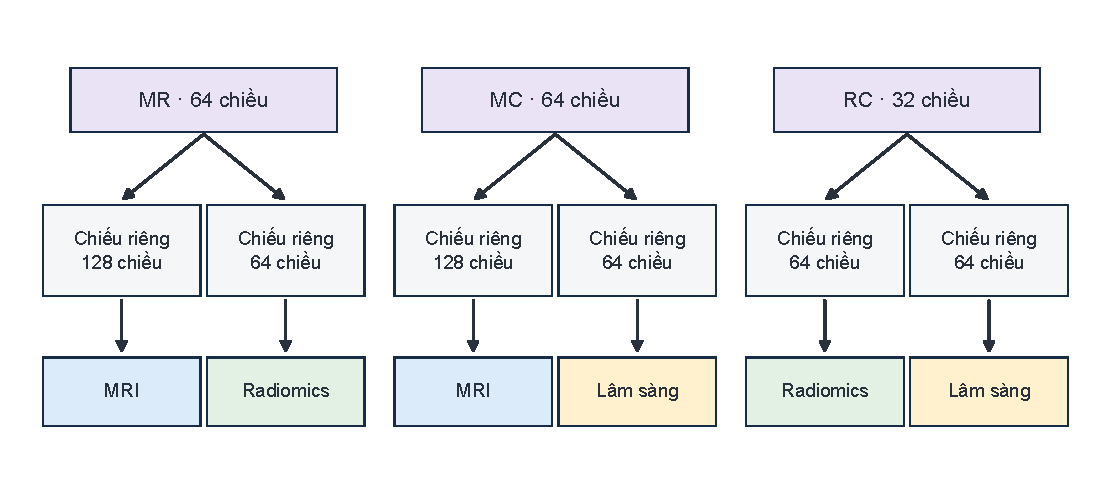
\includegraphics[width=\linewidth]{image/pair-update-routes.pdf}
\caption[Sáu nhánh cập nhật từ ba cặp tương tác]{Sáu nhánh cập nhật từ ba cặp tương tác đầy đủ về ba phương thức đích}
\label{fig:pair-update-routes}
\end{figure}

\subsection{Nén tham số tương tác bằng phân rã tensor CP}
\label{sec:cp-method}
Như đã phân tích ở Mục~\ref{sec:background-fusion}, lớp chiếu tuyến tính đầu tiên ngay sau phép tích ngoài tương đương với một tensor trọng số bậc ba $\mathcal W\in\mathbb R^{d_h\times d_x\times d_y}$ đòi hỏi tới $d_h d_x d_y + d_h$ tham số, rất dễ dẫn đến hiện tượng quá khớp trên tập huấn luyện 251 bệnh nhân. Nhằm giải quyết triệt để rào cản này, tôi áp dụng kỹ thuật phân rã tensor CP hạng $Q$ theo Công thức~(\ref{eq:cp-concept-math})--(\ref{eq:cp-hadamard}) \cite{carroll1970candecomp,kolda2009tensor,liu2018lowrank}: lớp song tuyến đầu tiên của mỗi cặp tương tác $k$ được thay thế bằng ba ma trận nhân tử $A\in\mathbb R^{d_x\times Q}$, $B\in\mathbb R^{d_y\times Q}$ (không sử dụng hệ số chệch) và $O\in\mathbb R^{d_h\times Q}$ (có hệ số chệch $b$):
\begin{align}
 u&=A^\top x,\qquad v=B^\top y,\qquad q=u\odot v,\label{eq:cp-lowrank}\\
 h&=Oq+b,\qquad E_k=\operatorname{PostMLP}_k(h).
 \label{eq:cpblock}
\end{align}
Trong đó, khối $\operatorname{PostMLP}_k$ giữ nguyên vẹn cấu trúc mạng phía sau gồm hàm kích hoạt GELU, Dropout 0.10, lớp tuyến tính $d_h\to d_o$ và lớp chuẩn hóa LayerNorm, xuất ra vectơ đặc trưng tương tác $E_k\in\mathbb R^{d_o}$ cho cặp $k\in\{\mathrm{MR},\mathrm{MC},\mathrm{RC}\}$ (cụ thể $E_{\mathrm{MR}}\in\mathbb R^{64}$, $E_{\mathrm{MC}}\in\mathbb R^{64}$ và $E_{\mathrm{RC}}\in\mathbb R^{32}$). Thiết kế này bảo đảm tính công bằng tuyệt đối trong so sánh thực nghiệm: biến thể CP chỉ can thiệp thay đổi đúng lớp song tuyến đầu tiên (Hình~\ref{fig:cp-block}) trong khi bảo toàn nguyên vẹn mọi tầng xử lý tiếp theo của Full Outer-Product. Số lượng tham số cần tối ưu của lớp tương tác đầu nhờ vậy được cắt giảm từ $d_h d_x d_y + d_h$ xuống chỉ còn $Q(d_x+d_y+d_h)+d_h$. Bảng~\ref{tab:cpconfig} tổng hợp cụ thể cấu hình kích thước và thứ hạng CP cho từng cặp (chọn $Q=8$ cho MR, MC và $Q=4$ cho RC do cặp RC có số chiều đầu ra nhỏ hơn).

\begin{figure}[H]
\centering
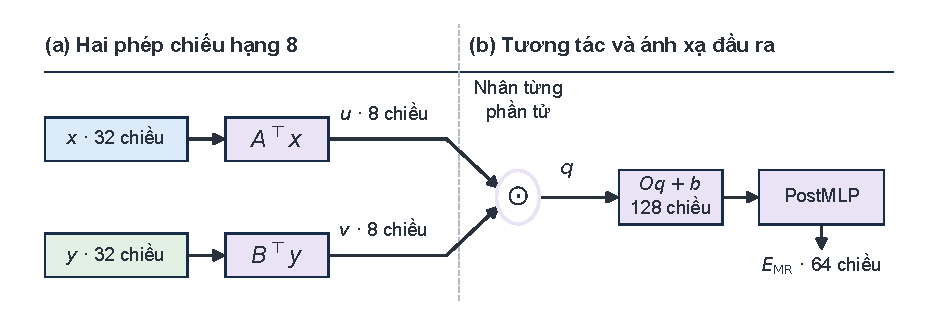
\includegraphics[width=\textwidth]{image/outer-vs-cp.pdf}
\caption[Khối tương tác CP hạng $Q=8$ cho cặp MR]{Luồng tính toán của khối tương tác CP hạng $Q=8$ cho cặp MR}
\label{fig:cp-block}
\end{figure}

\begin{table}[H]
\centering\small
\caption{Cấu hình kích thước và hạng CP theo từng cặp tương tác}
\label{tab:cpconfig}
\begin{tabular}{lccccc}
\toprule
Cặp & $(d_x,d_y)$ & Hạng $Q$ & Chiều ẩn $d_h$ & Đầu ra $d_o$ & RC-Free \\
\midrule
MR & $(32,32)$ & 8 & 128 & 64 & Giữ \\
MC & $(32,16)$ & 8 & 128 & 64 & Giữ \\
RC & $(32,16)$ & 4 & 64 & 32 & Loại \\
\bottomrule
\end{tabular}
\end{table}

\subsection{Truyền phần dư có cổng và cấu trúc tinh gọn RC-Free}
\label{sec:gated-routing}
\label{sec:rcfree-method}
Sau khi trích xuất được vectơ tương tác song tuyến $E_k\in\mathbb R^{d_o}$ từ mỗi cặp $k$ theo Công thức~(\ref{eq:cpblock}), bước xử lý then chốt tiếp theo là truyền ngược lượng thông tin tương tác này để bồi đắp và làm giàu cho biểu diễn gốc của hai phương thức thành phần. Ký hiệu $U_d$ là biểu diễn gốc của phương thức đích $d\in\{M,R,C\}$ (tương ứng với $U_M=M\in\mathbb R^{128}$, $U_R=R\in\mathbb R^{64}$ và $U_C=C\in\mathbb R^{64}$). Do mức độ tương tác giữa hai nguồn dữ liệu không phải lúc nào cũng mang lại giá trị như nhau ở mọi bệnh nhân hay mọi thời điểm thăm khám (chẳng hạn khi ảnh MRI bị mờ do nhiễu chuyển động hoặc các điểm lâm sàng bị thiếu phải điền giá trị ước lượng), mô hình đề xuất không cộng dồn trực tiếp $E_k$ mà dẫn truyền qua một nhánh phần dư có cổng điều tiết động $k\to d$ gồm ba khối xử lý liên hoàn (Hình~\ref{fig:route}):
\begin{enumerate}
\item \emph{Chiếu $E_k$ thành vectơ tương tác quy chiếu theo đích $\widehat E_{k\to d}$}: Vectơ tương tác chung $E_k$ chưa thể cộng trực tiếp vào biểu diễn gốc $U_d$, trước hết vì sự sai lệch về số chiều (chẳng hạn $E_{\mathrm{MR}}$ có 64 chiều trong khi đích MRI $U_M$ có 128 chiều), và quan trọng hơn là vì hai phương thức đích trong cùng một cặp đòi hỏi phải trích xuất hai góc nhìn thông tin bổ trợ khác nhau từ $E_k$. Do đó, trên mỗi nhánh dẫn truyền $k\to d$, tôi áp dụng một phép chiếu tuyến tính độc lập $W_{k\to d}$ (có độ chệch $b_{k\to d}$, không sử dụng phi tuyến) kết hợp lớp chuẩn hóa LayerNorm để biến đổi $E_k$ thành vectơ tương tác đã quy chiếu theo đích $\widehat E_{k\to d}$, có kích thước hoàn toàn tương thích với $U_d$:
\begin{equation}
 \widehat E_{k\to d}=\LN_{k\to d}(W_{k\to d}E_k+b_{k\to d}).
 \label{eq:target-projection}
\end{equation}
\item \emph{Cổng điều tiết động $g_{k\to d}\in(0,1)$ theo từng mẫu}: Cơ chế cổng tiếp nhận đồng thời cả biểu diễn gốc đã chuẩn hóa và vectơ tương tác đã quy chiếu nhằm quyết định mức độ mở cổng linh hoạt cho từng lần khám thông qua mạng MLP ẩn 32 chiều (khởi tạo trọng số Xavier \cite{glorot2010understanding}, hệ số chệch ban đầu đặt bằng 0) kết thúc bằng hàm kích hoạt sigmoid:
\begin{equation}
 g_{k\to d}=\sigma\!\left(
 w_{k\to d}^{\top}\operatorname{GELU}\!\left[
 V_{k\to d}\bigl(\LN_d^{\rm gate}(U_d)\concat\widehat E_{k\to d}\bigr)
 +a_{k\to d}\right]+c_{k\to d}\right).
 \label{eq:dynamic-gate}
\end{equation}
Việc sử dụng hàm sigmoid độc lập cho từng nhánh (thay vì áp dụng softmax ràng buộc tổng bằng 1) cho phép các nhánh có thể cùng mở rộng khi thông tin bổ trợ có độ tin cậy cao, hoặc chủ động khép chặt về 0 khi phát hiện tín hiệu bị nhiễu.
\item \emph{Hệ số tỷ lệ toàn cục $\lambda_{k\to d}$}: Một tham số vô hướng được học chung trên toàn tập dữ liệu (khởi tạo tại giá trị $0.1$ và không áp đặt ràng buộc dấu), đóng vai trò điều chỉnh biên độ và định hướng tương quan tổng thể của nhánh tương tác.
\end{enumerate}

\begin{figure}[H]
\centering
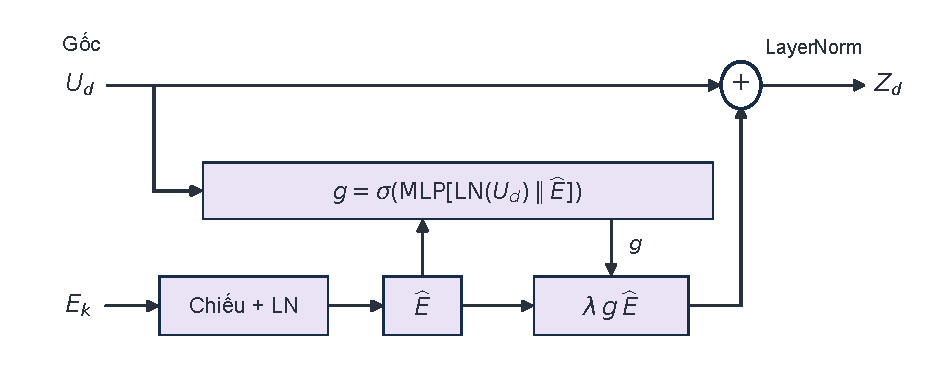
\includegraphics[width=\textwidth]{image/gated-residual-route.pdf}
\caption{Cấu trúc một nhánh phần dư có cổng điều tiết động}
\label{fig:route}
\end{figure}

Biểu diễn của phương thức đích $d$ sau khi tiếp nhận phần dư từ tập các cặp tương tác đang hoạt động $\mathcal P(d)$ được chuẩn hóa qua lớp LayerNorm độc lập:
\begin{equation}
 Z_d=\LN_d^{\rm out}\!\left(
 U_d+\sum_{k\in\mathcal P(d)}\lambda_{k\to d}\,g_{k\to d}\,\widehat E_{k\to d}
 \right).
 \label{eq:ours-residual}
\end{equation}
Ba tầng LayerNorm trong (\ref{eq:target-projection})--(\ref{eq:ours-residual}) sở hữu bộ tham số độc lập hoàn toàn \cite{ba2016layernorm}. Khi cổng điều tiết $g_{k\to d}$ triệt tiêu về 0, nhánh tương tác sẽ tắt hoàn toàn và biểu diễn đầu ra bảo toàn trọn vẹn đặc trưng gốc $\LN_d^{\rm out}(U_d)$.

Mô hình Full CP tiêu chuẩn duy trì cả ba cặp tương tác MR, MC, RC cùng trọn vẹn sáu nhánh phần dư. Tuy nhiên, xuất phát từ bản chất đặc trưng radiomics vốn được tính toán trực tiếp từ ảnh MRI, việc duy trì thêm tương tác trực tiếp giữa radiomics và lâm sàng (cặp RC) nhiều khả năng tạo ra sự dư thừa biểu diễn khi ảnh MRI vốn dĩ đã kết nối trực tiếp với cả hai phương thức này. Dựa trên nhận định đó, tôi đề xuất kiến trúc tinh giản \textbf{RC-Free}: loại bỏ hoàn toàn khối tương tác RC, lấy MRI làm nút trung tâm kết nối cho hai cặp MR và MC (cùng có hạng phân rã $Q=8$), qua đó tinh giản số nhánh phần dư có cổng từ sáu xuống còn bốn nhánh mà vẫn duy trì đầy đủ cả ba nguồn dữ liệu đầu vào (Hình~\ref{fig:rcfree-update}).

\begin{figure}[H]
\centering
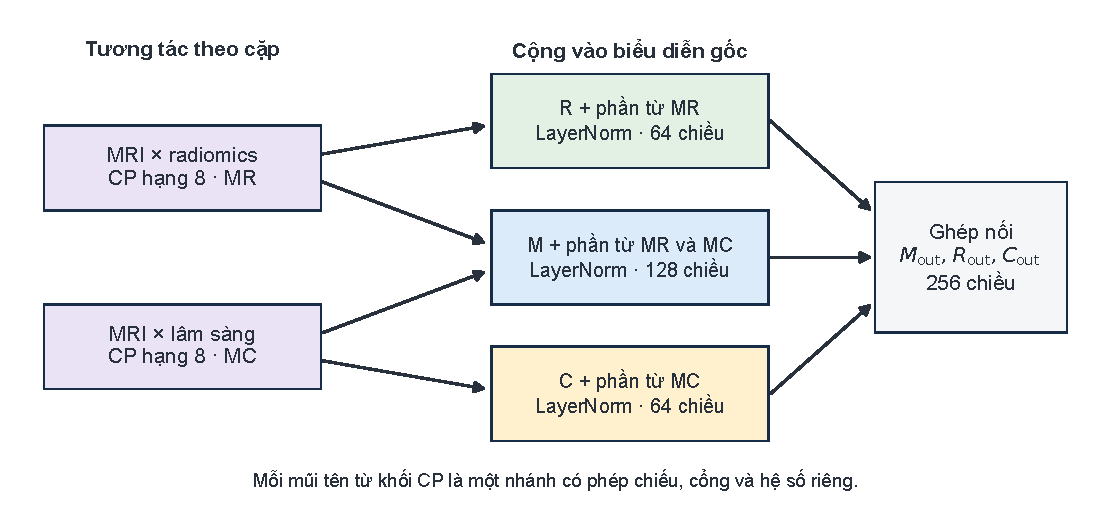
\includegraphics[width=\linewidth]{image/rcfree-update.pdf}
\caption{Bốn nhánh cập nhật đặc trưng trong kiến trúc RC-Free}
\label{fig:rcfree-update}
\end{figure}

Đặt $D_{k\to d}=\lambda_{k\to d}\,g_{k\to d}\,\widehat E_{k\to d}$, ba biểu diễn sau cập nhật của RC-Free có dạng:
\begin{align}
 M_{\rm out}&=\LN_M^{\rm out}(M+D_{(\mathrm{MR}\to M)}+D_{(\mathrm{MC}\to M)}),\label{eq:rcfree-first}\\
 R_{\rm out}&=\LN_R^{\rm out}(R+D_{(\mathrm{MR}\to R)}),\\
 C_{\rm out}&=\LN_C^{\rm out}(C+D_{(\mathrm{MC}\to C)}).
 \label{eq:rcfree-residual}
\end{align}
Ba vectơ sau cập nhật gồm $M_{\rm out}\in\mathbb R^{128}$, $R_{\rm out}\in\mathbb R^{64}$ và $C_{\rm out}\in\mathbb R^{64}$ được ghép nối thành vectơ 256 chiều rồi đưa qua lớp $\operatorname{MLP}_{\rm out}$ ($256\to128$, tương tự như Công thức~(\ref{eq:concat})) để thu được biểu diễn hợp nhất $F_t\in\mathbb R^{128}$ cho lần khám thứ $t$. Nhờ bảo toàn cố định kích thước đầu ra 128 chiều này, mọi biến đổi trong tập cấu hình tương tác cặp đều không làm xáo trộn các tầng xử lý chuỗi thời gian cũng như đầu dự báo sống còn phía sau.

\section{Mô hình thời gian và hàm mục tiêu Cox}
\label{sec:temporal-method}
\label{sec:training-method}
Chuỗi ba biểu diễn đa phương thức $F_t\in\mathbb R^{128}$ ($t=1,2,3$) cùng khoảng biến thiên thời gian thực tế giữa hai lần chụp liên tiếp $\Delta t_t=(s_t-s_{t-1})/365.25$ (tính theo năm, quy ước $\Delta t_1=0$) được đưa vào khối xử lý thời gian một lớp một chiều (Hình~\ref{fig:temporal}).

Áp dụng kiến trúc T-LSTM của Baytas và cộng sự \cite{baytas2017patient} với kích thước trạng thái ẩn 128 chiều, tại bước thời gian $t$, trạng thái bộ nhớ trước đó $c_{t-1}$ được phân rã thành thành phần ngắn hạn $c_{t-1}^{S}$ (được điều tiết suy giảm theo hàm trọng số $\gamma_t$ nghịch biến với $\Delta t_t$) và thành phần dài hạn bền vững $c_{t-1}^{L}$:
\begin{align}
 c_{t-1}^{S}&=\tanh(W_Sc_{t-1}+b_S),\qquad
 c_{t-1}^{L}=c_{t-1}-c_{t-1}^{S},\label{eq:tlstm-first}\\
 \gamma_t&=\frac{1}{\log(e+\Delta t_t)},\qquad
 c_{t-1}^{*}=c_{t-1}^{L}+\gamma_t c_{t-1}^{S}.
 \label{eq:tlstm-memory}
\end{align}
Trạng thái bộ nhớ hiệu chỉnh $c_{t-1}^{*}$ tiếp tục được tổng hợp qua các cổng quên $f_t$, cổng vào $i_t$, cổng ra $o_t$ và bộ nhớ ứng viên $\widetilde c_t$ chuẩn mực của LSTM (được tính toán từ $F_t$ và $h_{t-1}$):
\begin{equation}
 c_t=f_t\odot c_{t-1}^{*}+i_t\odot\widetilde c_t,
 \qquad h_t=o_t\odot\tanh(c_t).
 \label{eq:tlstm-state}
\end{equation}
(Nếu một lần khám bị đánh dấu không hợp lệ, mạng giữ nguyên trạng thái trước đó; trong nhóm dữ liệu này cả ba lần khám của mọi cá thể đều hợp lệ.)

\begin{figure}[H]
\centering
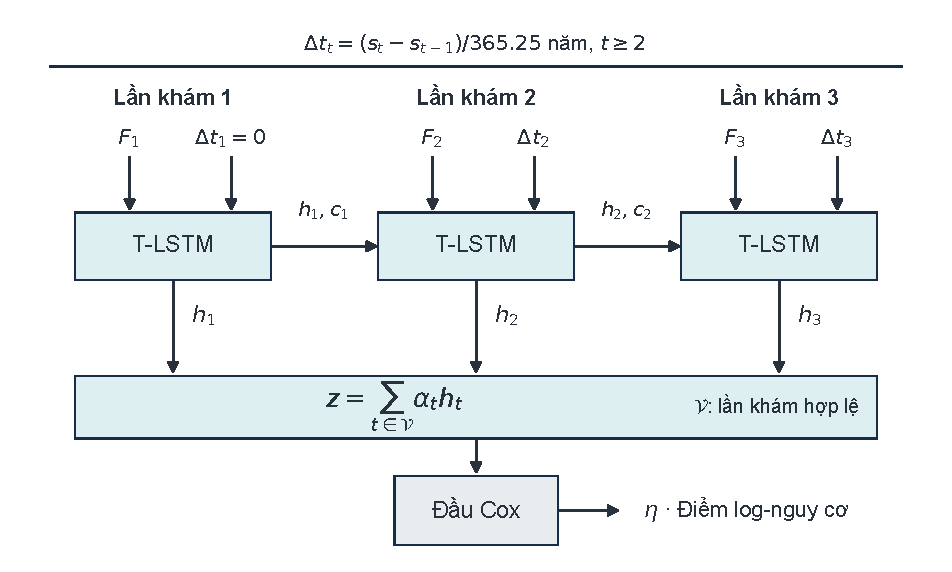
\includegraphics[width=\textwidth]{image/temporal-model.pdf}
\caption{Khối thời gian T-LSTM, attention cộng và đầu dự báo Cox}
\label{fig:temporal}
\end{figure}

Tiếp theo, cơ chế attention cộng (Công thức~(\ref{eq:additive-attention}) theo Yang và cộng sự \cite{yang2016hierarchical}) dùng phép chiếu $128\to64\to1$ để gán trọng số $\alpha_t$ cho từng lần khám hợp lệ trong tập $\mathcal V$:
\begin{equation}
 e_t=v_a^\top\tanh(W_a h_t+b_a),\qquad
 \alpha_t=\frac{\exp(e_t)}{\sum_{j\in\mathcal V}\exp(e_j)},\qquad
 z=\sum_{t\in\mathcal V}\alpha_t h_t.
 \label{eq:temporal-attention}
\end{equation}
Từ biểu diễn dọc $z\in\mathbb R^{128}$, một khối MLP đầu ra ($128\to64$ với GELU và Dropout 0.30, rồi tuyến tính $64\to1$) ước lượng điểm log-nguy cơ $\eta_i\in\mathbb R$ trong mô hình Cox~(\ref{eq:cox-hazard}). Mạng được huấn luyện bằng đối log-hợp lý riêng phần Cox (Công thức~(\ref{eq:cox-loss})) lấy trung bình trên $N_e$ biến cố quan sát trong lô, xử lý các ca trùng thời điểm theo xấp xỉ Breslow \cite{breslow1974covariance}:
\begin{equation}
 \mathcal L_{\rm Cox}=-\frac{1}{N_e}\sum_k
 \left[\sum_{i\in\mathcal D_k}\eta_i
 -d_k\log\!\left(\sum_{j\in\mathcal R_k}\exp(\eta_j)\right)\right],
 \label{eq:cox-method}
\end{equation}
với $\mathcal D_k$ là tập các ca có biến cố tại mốc phân biệt $\tau_k$ ($d_k=|\mathcal D_k|$) và $\mathcal R_k=\{j:t_j\geq\tau_k\}$ là tập nguy cơ ngay trước $\tau_k$. Toàn bộ luồng tính xuôi của RC-Free được tóm tắt thống nhất trong Thuật toán~\ref{alg:rcfree-forward}.

\begin{algorithm}[H]
\caption{Luồng tính xuôi của mô hình RC-Free Pairwise Fusion}
\label{alg:rcfree-forward}
\small
\textbf{Đầu vào:} Chuỗi ba lần khám $(t=1,2,3)$ của một cá thể gồm ảnh MRI đã tiền xử lý, vectơ đặc trưng radiomics sau PCA (16 chiều), vectơ lâm sàng gồm chín giá trị và chín chỉ báo quan sát (18 chiều) và khoảng cách thời gian $\Delta t_t$ (với $\Delta t_1=0$).\\
\textbf{Đầu ra:} Điểm log-nguy cơ $\eta\in\mathbb R$ của cá thể.
\begin{enumerate}[leftmargin=1.2em,label=\arabic*.,itemsep=0.2em]
\item Với mỗi lần khám $t=1,2,3$:
\begin{enumerate}[leftmargin=1.2em,label=\alph*.,itemsep=0.15em]
\item Mã hóa ba nguồn đầu vào tại lần khám $t$ thành $M_t\in\mathbb R^{128}$, $R_t\in\mathbb R^{64}$, $C_t\in\mathbb R^{64}$ theo Mục~\ref{sec:preprocessing}; chiếu tuyến tính không hệ số chệch về $\widetilde M_t\in\mathbb R^{32}$, $\widetilde R_t\in\mathbb R^{32}$, $\widetilde C_t\in\mathbb R^{16}$ theo (\ref{eq:input-projection}).
\item Tính đặc trưng tương tác $E_{\mathrm{MR},t}\in\mathbb R^{64}$ từ $(\widetilde M_t,\widetilde R_t)$ và $E_{\mathrm{MC},t}\in\mathbb R^{64}$ từ $(\widetilde M_t,\widetilde C_t)$ bằng hai khối CP hạng $Q=8$ kèm MLP theo (\ref{eq:cp-lowrank})--(\ref{eq:cpblock}).
\item Với mỗi nhánh $k\to d\in\{\mathrm{MR}\to M,\mathrm{MR}\to R,\mathrm{MC}\to M,\mathrm{MC}\to C\}$, tính phép chiếu theo đích $\widehat E_{k\to d,t}$ theo (\ref{eq:target-projection}), cổng điều tiết $g_{k\to d,t}$ theo (\ref{eq:dynamic-gate}) và lượng bổ sung $D_{k\to d,t}=\lambda_{k\to d}\,g_{k\to d,t}\,\widehat E_{k\to d,t}$.
\item Cập nhật phần dư và chuẩn hóa theo (\ref{eq:rcfree-first})--(\ref{eq:rcfree-residual}) để thu được $M_{\mathrm{out},t}\in\mathbb R^{128}$, $R_{\mathrm{out},t}\in\mathbb R^{64}$ và $C_{\mathrm{out},t}\in\mathbb R^{64}$.
\item Ghép nối và ánh xạ thành biểu diễn hợp nhất tại lần khám $t$: $F_t=\operatorname{MLP}_{\mathrm{out}}(M_{\mathrm{out},t}\concat R_{\mathrm{out},t}\concat C_{\mathrm{out},t})\in\mathbb R^{128}$ theo (\ref{eq:concat}).
\end{enumerate}
\item Khởi tạo trạng thái ẩn và bộ nhớ bằng không; đưa chuỗi $(F_t,\Delta t_t)_{t=1}^3$ qua T-LSTM theo (\ref{eq:tlstm-first})--(\ref{eq:tlstm-state}) để thu được các trạng thái ẩn $h_1,h_2,h_3\in\mathbb R^{128}$.
\item Tính trọng số attention $\alpha_t$ và biểu diễn tổng hợp chuỗi $z=\sum_{t=1}^3\alpha_t h_t\in\mathbb R^{128}$ theo (\ref{eq:temporal-attention}).
\item Đưa $z$ qua khối MLP dự báo sống còn Cox ($128\to64\to1$) ở Mục~\ref{sec:training-method} để xuất điểm log-nguy cơ $\eta$.
\end{enumerate}
\end{algorithm}


\section{Đánh giá xếp hạng và phân tầng nguy cơ}
\label{sec:survival-evaluation}
Một mô hình sống còn cần được đánh giá đồng thời ở ba khía cạnh bổ trợ nhau (Hình~\ref{fig:evaluation-map}): khả năng xếp hạng toàn cục (C-index), khả năng chia nhóm nguy cơ theo thời gian (Kaplan--Meier) và độ phân biệt tại các thời hạn lâm sàng cụ thể (IPCW-AUC). Toàn bộ đánh giá được tính trên điểm nguy cơ $\eta_i$ xuất từ ba mô hình RC-Free đã cố định trọng số (ứng với ba lần khởi tạo ngẫu nhiên).

\begin{figure}[H]
\centering
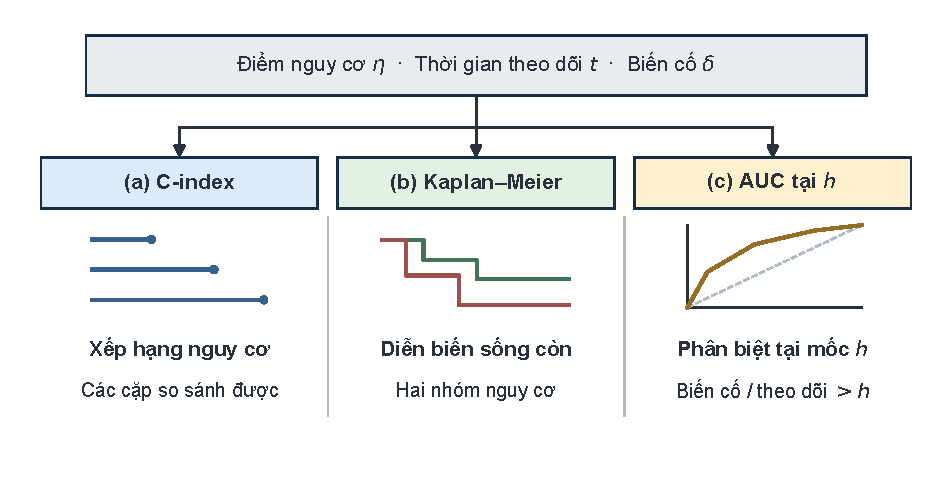
\includegraphics[width=\textwidth]{image/evaluation-map.pdf}
\caption{Ba góc nhìn đánh giá và phân tầng điểm nguy cơ sống còn}
\label{fig:evaluation-map}
\end{figure}

\subsection{Chỉ số đồng thuận C-index}
Harrell's C-index \cite{harrell1996multivariable} đo tỷ lệ các cặp cá thể có thể so sánh được ($t_i<t_j$, $\delta_i=1$) mà mô hình xếp đúng người gặp biến cố sớm hơn có điểm nguy cơ cao hơn ($\eta_i>\eta_j$). Giá trị 0.5 tương ứng đoán ngẫu nhiên và 1.0 là xếp hạng hoàn hảo. Tập xác thực có 480 cặp so sánh hợp lệ và tập kiểm tra hậu nghiệm có 528 cặp; kết quả được báo cáo dưới dạng trung bình $\pm$ độ lệch chuẩn mẫu (SD) qua ba lần khởi tạo.

\subsection{Phân tầng Kaplan--Meier theo nhóm nguy cơ đồng thuận}
Để kiểm tra xem điểm nguy cơ liên tục có tách được hai nhóm diễn biến khác nhau hay không, tôi dùng \emph{trung vị điểm nguy cơ trên tập huấn luyện} làm ngưỡng phân nhóm (tránh dùng thông tin từ tập xác thực hay kiểm tra): người vượt ngưỡng thuộc nhóm nguy cơ cao, ngược lại thuộc nhóm nguy cơ thấp. Để giảm phụ thuộc vào một lần khởi tạo đơn lẻ, nhãn nhóm cuối cùng được xác định theo \emph{đồng thuận đa số} (xếp vào nhóm nguy cơ cao nếu ít nhất 2 trong 3 lần khởi tạo xếp vào nhóm này).

Với hai nhóm thu được, đường cong Kaplan--Meier \cite{kaplan1958nonparametric} ước lượng xác suất chưa xảy ra biến cố theo thời gian, vẽ kèm khoảng tin cậy 95\%, dấu kiểm duyệt và bảng số người còn nguy cơ tại các mốc 0, 2, 3 và 5 năm. Khác biệt giữa hai đường cong được kiểm định bằng phép kiểm định log-rank \cite{mantel1966survival}, đồng thời hồi quy Cox đơn biến ước lượng tỷ số nguy cơ (Hazard Ratio -- HR) cùng khoảng tin cậy 95\% trên toàn bộ thời gian theo dõi. Giả định nguy cơ tỷ lệ (PH) được kiểm tra bằng phần dư Schoenfeld chuẩn hóa theo Grambsch và Therneau \cite{grambsch1994proportional} (biến đổi thời gian theo thứ hạng).

\subsection{AUC phụ thuộc thời gian có trọng số IPCW tại 2, 3 và 5 năm}
Tại mỗi mốc thời hạn $h \in \{2, 3, 5\text{ năm}\}$, tôi đánh giá khả năng phân biệt giữa nhóm đã gặp biến cố tính đến $h$ ($\mathcal C_h=\{i:\delta_i=1,t_i\leq h\}$) và nhóm còn theo dõi vượt quá $h$ ($\mathcal D_h=\{j:t_j>h\}$) bằng AUC tích lũy/động \cite{hung2010time}. Vì những người bị kiểm duyệt trước $h$ không rõ trạng thái tại $h$, bỏ qua họ một cách trực tiếp sẽ gây thiên lệch; do đó mỗi ca biến cố được gán trọng số nghịch đảo xác suất chưa bị kiểm duyệt $w_i = 1/\widehat G(t_i)$ (IPCW) \cite{polsterl2020scikit,hung2010time}, với $\widehat G(\cdot)$ ước lượng bằng Kaplan--Meier trên tập huấn luyện dưới giả định kiểm duyệt độc lập với thời gian biến cố và đặc trưng \cite{sksurvauc}:
\begin{equation}
 \widehat{\operatorname{AUC}}(h)=
 \frac{\displaystyle\sum_{i\in\mathcal C_h}w_i
 \sum_{j\in\mathcal D_h}\kappa(\eta_i,\eta_j)}
 {\displaystyle |\mathcal D_h|\sum_{i\in\mathcal C_h}w_i},
 \qquad
 \kappa(a,b)=\begin{cases}
 1,&a>b,\\
 \tfrac12,&a=b,\\
 0,&a<b.
 \end{cases}
 \label{eq:ipcw-auc}
\end{equation}
Theo cài đặt chuẩn của \texttt{scikit-survival}, hai điểm nguy cơ chênh lệch không quá $10^{-8}$ được xem là đồng điểm \cite{sksurvauc}. Để tránh ngoại suy hàm kiểm duyệt khi thời gian theo dõi tối đa ở tập xác thực (18.26 năm) vượt tập huấn luyện (13.95 năm), thời gian đánh giá được chặn tại $h+\varepsilon$ (xác định bằng \texttt{nextafter}).
